%% Copyright (C) 2014 by Pascal Richter, Elena Botoeva, Richard Barnard, and Dirk Surmann
%% 
%% This file may be distributed and/or modified under the
%% conditions of the LaTeX Project Public License, either
%% version 2.0 of this license or (at your option) any later
%% version. The latest version of this license is in:
%% 
%% http://www.latex-project.org/lppl.txt
%% 
%% and version 2.0 or later is part of all distributions of
%% LaTeX version 2013/12/01 or later.
%% 

\documentclass[]{tikzposter} %Options for format can be included here

\usepackage{epsfig}
\usepackage{amsmath}
\usepackage{amssymb}
\usepackage{multicol}
\usepackage{caption}
\usepackage{amsthm}

\newtheorem*{theorem*}{Theorem}

\def\cparam{\mathbf{c}}
\def\R{\mathbb{R}}
\def\H{\mathbb{H}}
\def\N{\mathbb{N}}
\def\Z{\mathbb{Z}}
\def\Q{\mathbb{Q}}
\def\C{\mathbb{C}}
\def\P{\mathbb{P}}
\def\E{\mathbb{E}}
\def\c#1{\mathcal{#1}}
\def\r#1{\text{#1}}
\def\h#1{\widehat{#1}}
\def\b#1{\mathbb{#1}}
\def\t#1{\widetilde{#1}}
\def\on{\mathrm{On}}
\def\1{\mathbbold{1}}
\def\eps{\varepsilon}
\def\diff{\backslash}
\def\d{\mathrm{d}}
\def\pd{\partial}

\def\D{\mathbb{D}}

 % Title, Author, Institute
\title{Connecting distant points via random blobs}
\author{Frankie Higgs, \texttt{fh350@bath.ac.uk}}
\institute{\Large Department of Mathematical Sciences, University of Bath\\\LARGE Based on joint work with Mathew Penrose}
\titlegraphic{
\includegraphics[scale=2.5]{images/uob-logo-grey-transparent}}

 %Choose Layout
\usetheme{Simple}

\settitle{
\centering
\vspace{30pt}
\vbox{
	\resizebox{\linewidth-100pt}{!}{\bfseries \@title}
	\vspace{20pt}
	\begin{minipage}[c]{0.5\linewidth}
		\centering
		\huge
		\@author
		
		\vspace{15pt}
		%\Large
		\@institute
	\end{minipage}
	\begin{minipage}[c]{0.4\linewidth}
		\centering
		\@titlegraphic
	\end{minipage}
	\vspace{-80pt}
}	
}

\begin{document}

 % Title block with title, author, logo, etc.
\maketitle

\block{The ``random blob'' or Boolean model}{
	\begin{minipage}[c]{0.25\linewidth}
		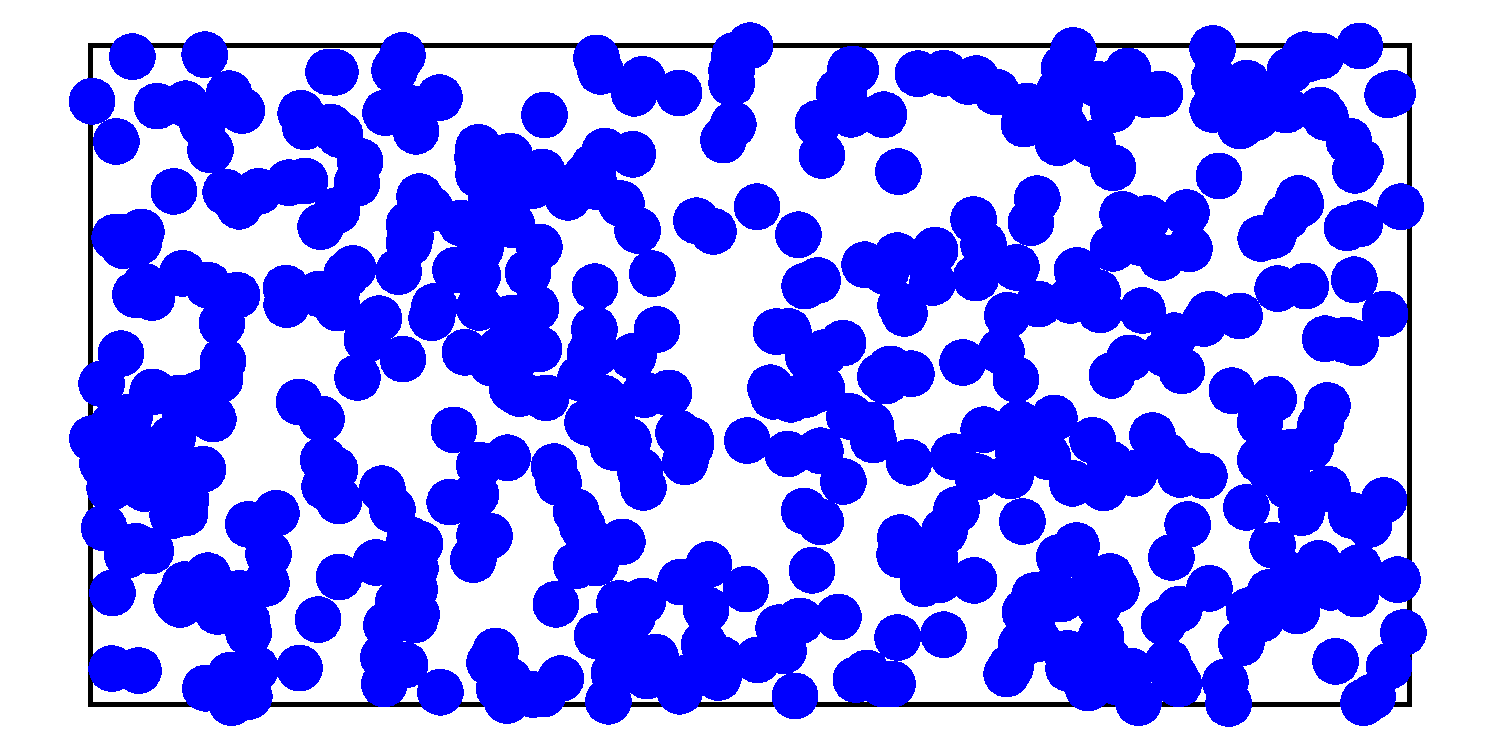
\includegraphics[width=\linewidth, trim=0 0 0 0, clip]{connection-diagram/boolean}
	\end{minipage}
	\begin{minipage}[c]{0.75\linewidth}
		The \emph{Boolean model} or \emph{random blob model}
		is the union of balls of radius $r$
		centred at the points of a point process $\mathcal{P}$ in a set $A$.
		%
		It is closely related to the \emph{random geometric graph},
		in which the points of $\mathcal{P}$ are vertices
		and edges join the pairs of points which are within distance $2r$.
		
		Suppose $A \subseteq \R^d$ is bounded,
		and $\mathcal{P}_\lambda$ is a homogeneous Poisson point process
		of intensity $\lambda$.
		If $\lambda = n / |A|$ so $\E[ \# \mathcal{P}_\lambda ] = n$
		(or if we replace $\mathcal{P}_\lambda$ with $n$ iid uniform points in $A$),
		we obtain the \emph{Boolean model} denoted $Z(n,r)$.
		We often choose $r = r_n$ by setting the parameter $\Lambda_n = n r_n^d$,
		as it is $\Lambda_n$ that determines many of the properties of $Z(n,r_n)$.
		%
		If $x \in A^\circ$ is at least distance $r_n$ from the boundary,
		then the expected number of balls which contain $x$
		is exactly proportional to $\Lambda_n$,
		and the probability $x \in Z(n,r_n)$ depends on $\Lambda_n$,
		for all $n$.
		%
		For a given sequence of $\Lambda_n$s, this makes the question of
		\emph{limiting behaviour}
		as $n \to \infty$ very interesting.
	\end{minipage}
}

\begin{columns}
 % FIRST column
\column{0.5}% Width set relative to text width
\block{Continuum percolation}{
	Suppose $A = \R^d$ or $\H := (0,\infty) \times \R^{d-1}$,
	fix $r = 1$
	and let $\mathcal{P}^A_\lambda$ be a homogeneous Poisson process of intensity $\lambda > 0$.
	%
	In this case, the Boolean model
	$Z^A_\lambda = \bigcup_{x \in \mathcal{P}_\lambda^A} B(x,1)$
	is normally referred to as
	\emph{continuum percolation}.
	%
	There are also many variants on continuum percolation,
	particularly when the balls have random radii:
	Meester and Roy's book Continuum Percolation
	is a very good introduction.
	
	As the name suggests,
	continuum percolation has many behaviours similar to discrete percolation.
	For example, we can define the \emph{percolation probability}
	\[
		\theta_A(\lambda) := \P_\lambda[\, 0 \text{ is in an unbounded component of $Z^A_\lambda$ }]
	\]
	and there is a non-trivial \emph{critical intensity}
	\[
		\lambda_c^A := \inf\{ \lambda > 0 : \theta_A(\lambda) > 0 \}.
	\]
	It is also known that $\lambda_c^{\H} = \lambda_c^{\R^d}$,
	so we will can just write $\lambda_c$ to denote the critical intensity.
	\begin{minipage}{\linewidth}
	\centering
	\begin{tikzfigure}
		\includegraphics[width=0.32\linewidth, trim=0 0 0 0, clip]{connection-diagram/phase-0.35}\hfill
		\includegraphics[width=0.32\linewidth, trim=0 0 0 0, clip]{connection-diagram/phase-0.36}\hfill
		\includegraphics[width=0.32\linewidth, trim=0 0 0 0, clip]{connection-diagram/phase-0.37}
	\end{tikzfigure}
	Three realisations of the Boolean model in $\R^2$ corresponding to continuum percolation
	with $\lambda = 0.35$, $\lambda = 0.36$ and $\lambda = 0.37$ respectively.
	Each component is coloured according to its size (darker components are larger).
	Numerical studies show $\lambda_c \approx 0.36$.
	\vspace{-50pt}
	\end{minipage}
}

\block{Connection events}{
	Suppose $A$ has a complicated geometry.
	As long as the boundary is smooth,
	the Boolean model near $\partial A$
	should ``look like'' a rescaled verison of continuum percolation in $\H$.
	Can we relate events inside $A$ to continuum percolation
	events in the canonical sets $\R^d$ and $\H$?
	
	For example, suppose $x, y \in \overline{A}$.
	Let $\{ x \leftrightarrow y \text{ in } Z(n,r) \}$ denote the event
	that $x$ and $y$ are in the same connected component of the Boolean model.
	
	\begin{theorem*}[2024+, H. and Penrose]
		Suppose $A \subseteq \R^d$ is open, connected and has a $C^2$ boundary.
		Let $x, y$ be two distinct points on $\partial A$
		and let $\lambda \in (0,\infty) \setminus \{ \lambda_c \}$.
		If $\Lambda_n \to \lambda$ as $n \to \infty$,
		then
		\[
			\lim_{n\to\infty} \P[ x \leftrightarrow y \text{ in } Z(n,r_n)]
			=
			\theta_{\H}(\lambda)^2.
		\]
	\end{theorem*}
	\vspace{-2cm}
}
\begin{subcolumns}

\subcolumn{0.55}
\block{Boundary effects}{
	A similar result with $x,y$ chosen \emph{uniformly} in $[0,1]^2$
	(so almost surely in the interior of the square)
	was proven in 2022 by Penrose.
	
	If $A$ is any polytope,
	an analogous result to our recent theorem for points \emph{on the boundary}
	should also	hold, but comparing to events from continuum percolation in \emph{cones}.
	
	To work near the boundary, we fit the part of $\partial A$ near $x$
	between the two tangent sphere meeting the boundary at $x$.
	Then we can relate events on one side of the tangent plane
	to continuum percolation in $\H$.
}

\subcolumn{0.45}
\block{What about $\lambda_c$?}{
	We required that $\lambda \not= \lambda_c$ for our result.
	Why?
	
	It is unknown whether $\theta_{\R^d}(\lambda_c) = 0$
	except when $d=2$ and $d \geq 11$.
	If $\theta(\lambda_c) > 0$,
	this would have a number of implications for percolation.
	In particular, points which \emph{are} in the same component
	may not be connected inside quite a large box.
	So even if $x$ and $y$ are in huge components, they may not meet inside $A$.
}
\end{subcolumns}


 % SECOND column
\column{0.50}

\block{Renormalisation}{
	To construct long-range connections in the Boolean model,
	we define a finite grid of balls with spacing $M r_n$ (for some large constant $M$)
	and construct a \emph{site percolation} model on this grid
	using the Boolean model.
	
	A ``good'' vertex is the centre of a ball of radius $K r_n$
	which intersects a unique large component of $Z(n,r_n)$
	\emph{inside a box of side lengths $2dM$}
	which also intersects all neighbouring balls in the grid.
	
	\begin{minipage}[c]{0.25\linewidth}
		By choosing $K$, $M$ and other parameters appropriately,
		we can ensure most balls in the grid are good.
		Since all these events occur \emph{inside a box},
		the dependence structure of the ``good events'' is simple.
	\end{minipage}
	\begin{minipage}[c]{0.75\linewidth}
		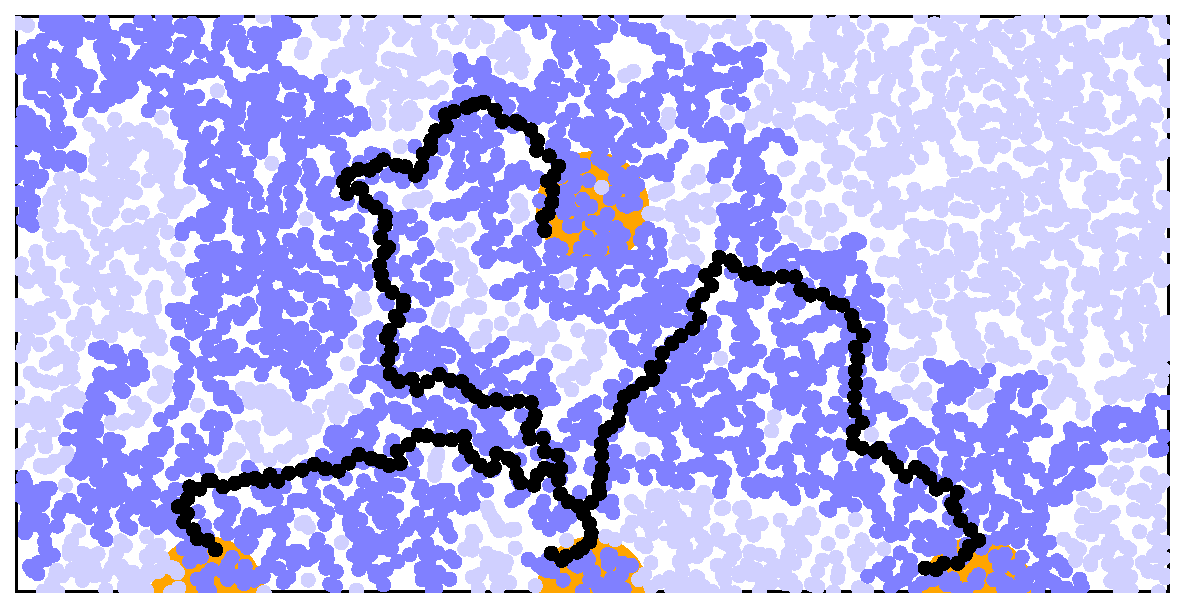
\includegraphics[width=\linewidth, trim=0 0 0 0, clip]{connection-diagram/renormalisation}
	\end{minipage}

	If you can prove that appropriate choices of $K$ and $M$ can be made
	under the assumption that $\theta_\H(\lambda) > 0$
	(rather than $\lambda > \lambda_c$),
	then this implies $\theta_{\R^d}(\lambda_c) = 0$,
	which is a major open problem in percolation.
	Left here as an exercise for the reader...
}

\begin{subcolumns}
\subcolumn{0.7}
\block{}{
	\centering
	\begin{tikzpicture}
	\node at (0,0) {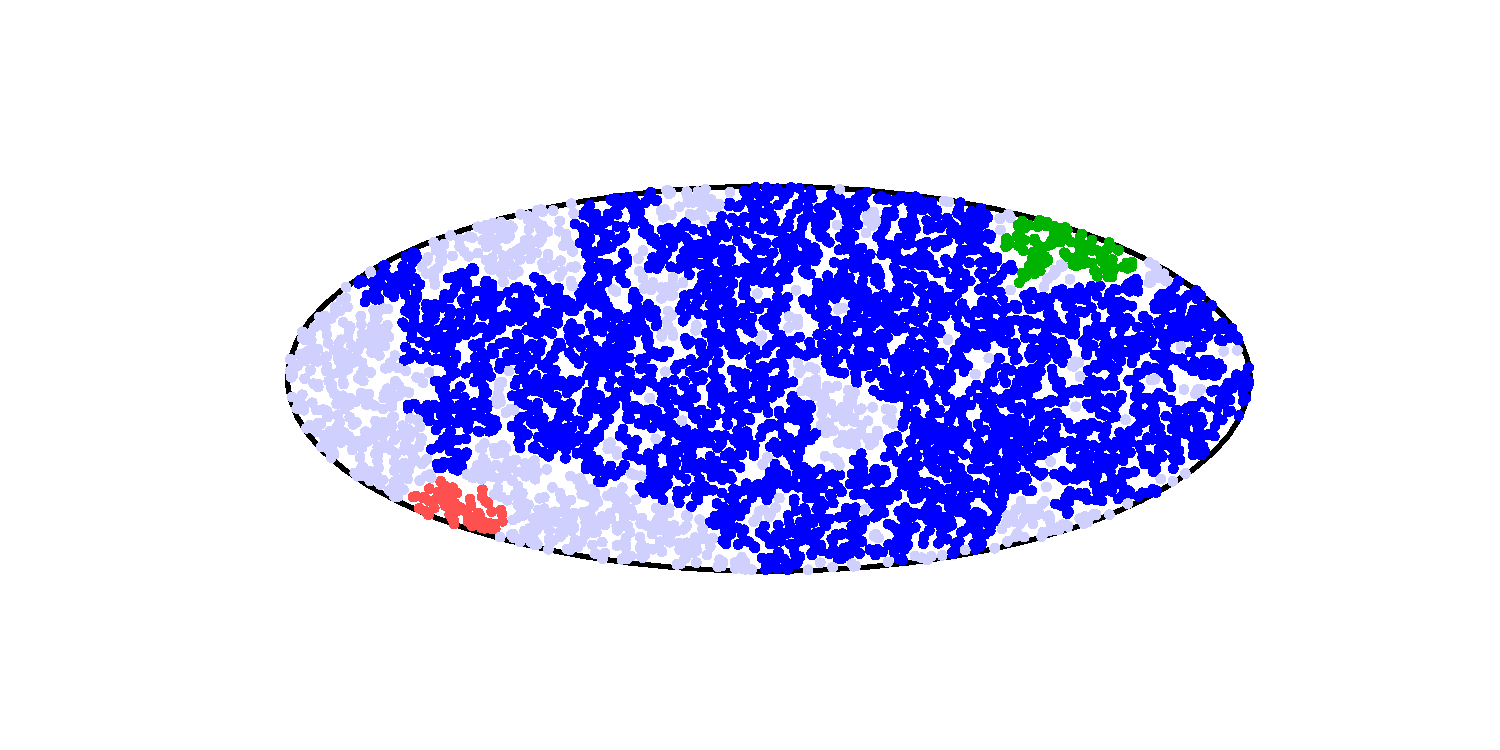
\includegraphics[width=1.0\linewidth, trim=130 80 115 85, clip]{connection-diagram/neither_percolates}};
	\node at (-8.75,-4.25) {$x$};
	\node at ( 9.0, 4.25) {$y$};
	\end{tikzpicture}
	When $\lambda > \lambda_c$,
	there will be a giant component.
	Above,
	neither $x$ nor $y$
	is contained in the giant component.
	\begin{tikzpicture}
	\node at (0,0) {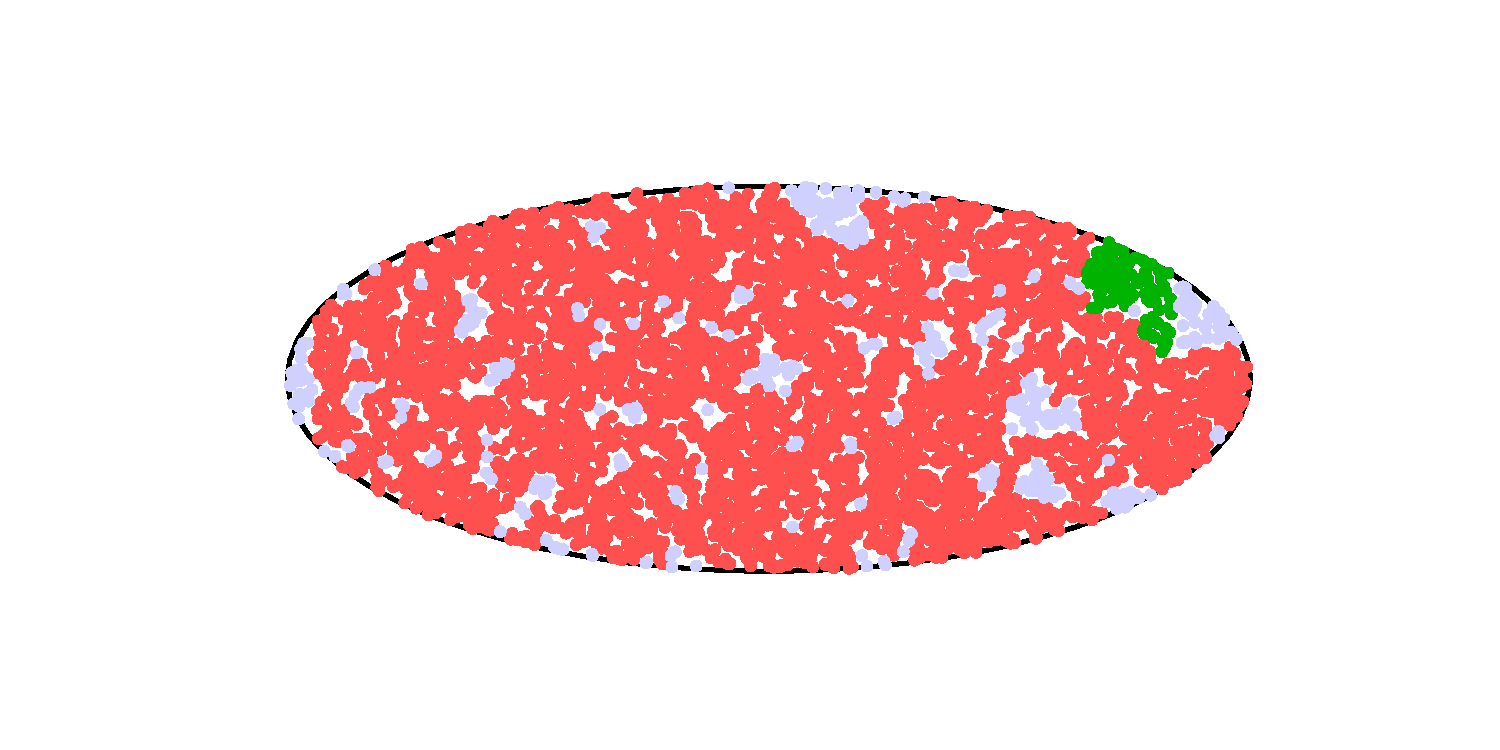
\includegraphics[width=1.0\linewidth, trim=130 80 115 50, clip]{connection-diagram/x_percolates}};
	\node at (-9.0,-5.0) {$x$};
	\node at ( 9.25, 3.25) {$y$};
	\end{tikzpicture}
	$x$ is in the giant component,
	but $y$ is not.
	\begin{tikzpicture}
	\node at (0,0) {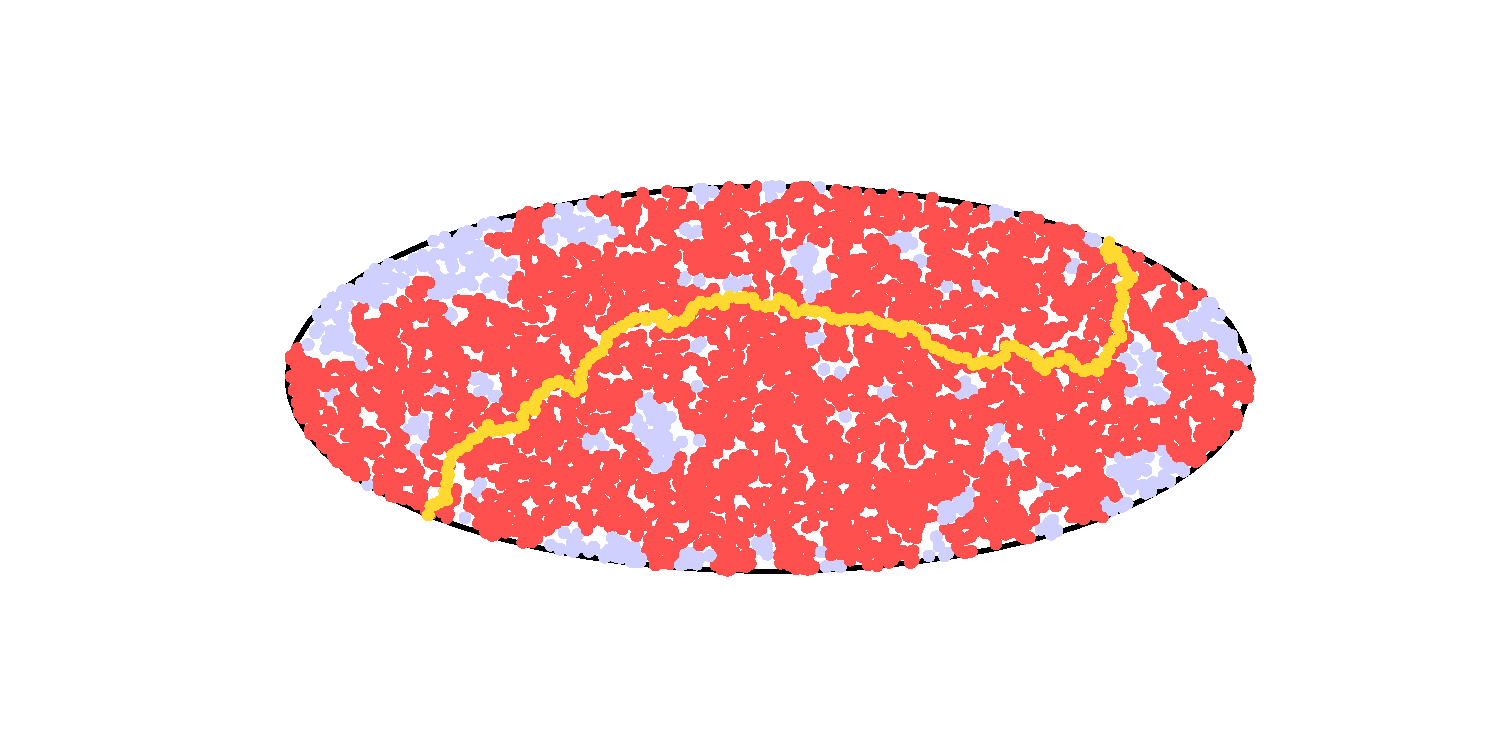
\includegraphics[width=1.0\linewidth, trim=130 80 115 50, clip]{connection-diagram/simple-path}};
	\node at (-9.0,-5.0) {$x$};
	\node at ( 9.25, 3.25) {$y$};
	\end{tikzpicture}
	$x$ and $y$ are connected via the giant component.
}

\subcolumn{0.3}
\block{Extensions}{
	There are some very easy extensions
	which would follow directly from our methods.
	For example,
	the probability that a collection of $k$ distinct points
	are all in a single component
	should have a similar limit.
	
	A more interesting extension is the question of whether $x$ and $y$
	are in the same component of $\overline{A} \setminus Z(n,r)$.
	This \emph{vacancy percolation} is very interesting,
	and quite challenging.
	For example, there is no lower bound on the size of a component,
	and the component can have much more complicated shapes
	than those of $Z(n,r)$.
}

\end{subcolumns}
\block{What else can $\Lambda_n$ do?}{
	If $\Lambda_n = \Theta(\log n)$,
	other events like coverage $\{A \subseteq Z(n,r_n)\}$,
	connectivity of $Z(n,r_n)$
	and interesting properties of the homology of $Z(n,r_n)$ become non-trivial.
}
\end{columns}
\end{document}

\endinput
%%
%% End of file `tikzposter-template.tex'.
